\documentclass[10pt,journal,compsoc]{IEEEtran}

    \usepackage[pdftex]{graphicx}    
    \usepackage{cite}
    \hyphenation{op-tical net-works semi-conduc-tor}
    
    
    \begin{document}
    
    \title{Mobile Robot's Position and Orientation using Adaptive Monte Carlo Localization}
    
    \author{Trim Bresilla}
    
    \markboth{Localization project, Robotics Nanodegree Program, Udacity}%
    {}
    \IEEEtitleabstractindextext{%
    
    \begin{abstract}
    This work describes one of the challenges in localization of mobile robotic. Using different probabilistic techniques and algorithms served by Robotic Operating System, by filtering noisy sensor data, we are able to get precise pose of mobile robot. To do that, we use a package - AMCL - that goes through sensor readings and estimates the pose and orientation of the mobile robot. Movebase, another ROS package takes those readings and uses for navigation stack, that the robot reaches the destination. While all this is run through the Gazebo simulator with its own physics engine (that utilizes collision, visuals etc...). By tunning AMCL's parameters we can estimate very accurately robot's pose and orientation and then navigate to goal position without any collision.
    \end{abstract}
    
    % Note that keywords are not normally used for peerreview papers.
    \begin{IEEEkeywords}
    Robot, IEEEtran, Udacity, \LaTeX, Localization.
    \end{IEEEkeywords}}
    
    
    \maketitle
    \IEEEdisplaynontitleabstractindextext
    \IEEEpeerreviewmaketitle
    \section{Introduction}
    \label{sec:introduction}
    
    \IEEEPARstart{L}{ocalisation} is one of the biggest challenge in mobile robotic. Determining robot's pose in mapped environment is very important for later activities like path-planning, manipulation etc. This is highly important in environment where precision very high (manufacturing). Using different probabilistic algorithms to filter noise from sensors (IMU, Rotary Encoders, Range-filters or 3D cameras).
    
    %example for inserting image
    \begin{figure}[thpb]
          \centering
          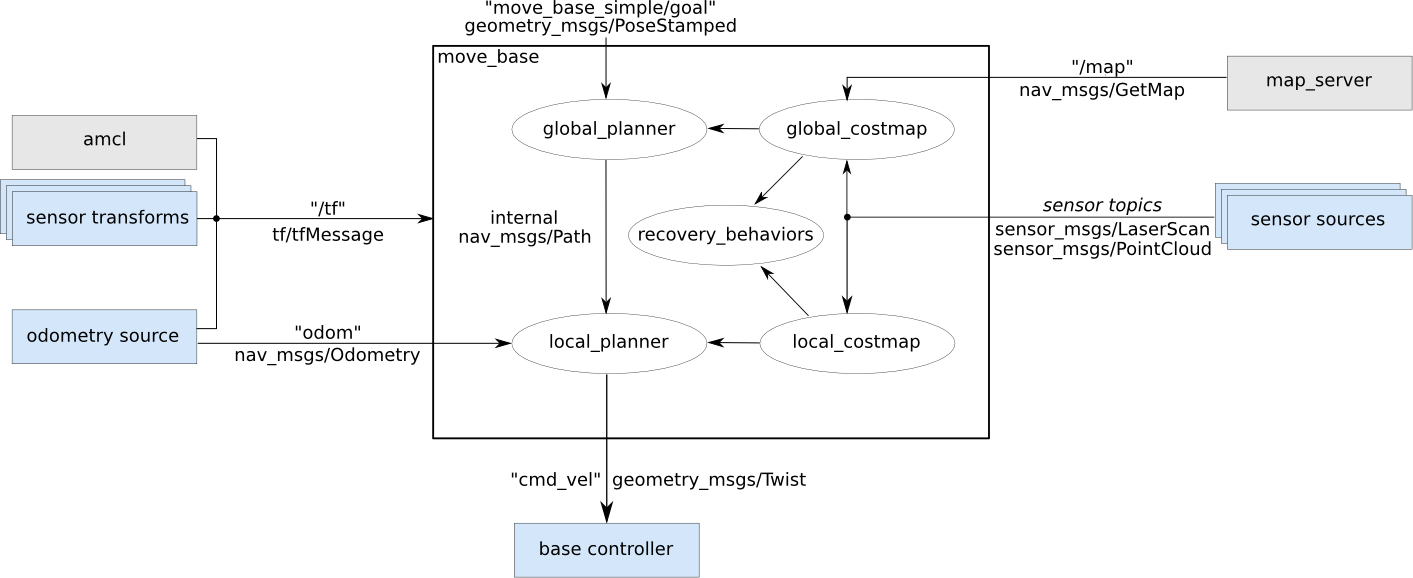
\includegraphics[width=\linewidth]{overview_tf.png}
          \caption{Naigation Stack Setup}
          \label{fig:robot1}
    \end{figure}

    %example for building table
    \begin{table}[h]
    \caption{Table}
    \label{table_example}
    \begin{center}
    \begin{tabular}{|c||c|}
    \hline
    One & Two\\
    \hline
    Three & Four\\
    \hline
    \end{tabular}
    \end{center}
    \end{table}
    
    
    
    \section{Background}
    At this stage, you should begin diving into the technical details of your approach by explaining to the reader what are the characteristics of the filters, what localization method was chosen, and the reason that it was selected (i.e. particle filters). 
    This should be factual and authoritative, meaning you should not use language such as "I think this will work" or "Maybe Monte Carlo Localization with these parameters is better...". Instead, focus on items similar to, "Adaptive Monte Carlo Localization was chosen because..."

    \subsection{Kalman Filters}
    Briefly describe Kalman filters. Explain how they work and why they are used for localization. Additionally, discuss the drawbacks of linear Kalman filters and how Extended Kalman Filters (EKFs) help resolve some of these issues.
    
    \subsection{Particle Filters}
    Briefly explain what a particle filter is, how it is used, and why it is useful.
    
    \subsection{Comparison / Contrast}
    Explain the benefits and disadvantages of using a Kalman Filter / Particle Filter. Why would you use one over the other? Also inform the reader that the work presented here will be using only particle filters. 
    
    %example for Bullet point list
    \begin{itemize}
    \item example 1
    \item example 2
    \end {itemize}
    
    %example for numbered list
    \begin{enumerate}
    \item example 1
    \item example 2
    \end{enumerate}
    
    \section{Simulations}
    This section should discuss the performance of robots in simulation. Items to include are the robot model design, packages used, and the parameters chosen for the robot to properly localize itself. The information provided here is critical if anyone would like to replicate your results. After all, the intent of reports such as these are to convey information and build upon ideas so you want to ensure others can validate your process.
    You should have at least two images here: one that shows your standard robot used in the first part of the project, and a second robot that you modified / built that is different from the first robot. Remember to watermark all of your images as well. 
    
    \subsection{Achievements}
    You should describe what you achieved for localization in the project with the benchmark model and your own model. Includes charts and graphs show how parameters affect your performance. 
    
    % Robot Models
    \subsection{Benchmark Model}
    \subsubsection{Model design}
    The Robot's design considerations should include: the size of the robot, the layout of sensors. This information can be shown in the form of a chart / table.
    
    \subsubsection{Packages Used}
    The packages used in the project should be specified as well as the topics received and published; the services it used and provided should also be addressed. 
    
    \subsubsection{Parameters}
    Localization parameters in the AMCL node should be described, as well as move\_base parameters in the configuration file. You should be able to clearly demonstrate your understanding of the impact of these parameters.
    
    \subsection{Personal Model}
    % ditto
    \subsubsection{Model design}
    \subsubsection{Packages Used}
    \subsubsection{Parameters}
    
    
    \section{Results}
    Present an unbiased view of your robot's performance and justify your stance with facts. Do the localization results look reasonable? What is the duration for the particle filters to converge? How long does it take for the robot to reach the goal? Does it follow a smooth path to the goal? Does it have unexpected behavior in the process? \\
    For demonstrating your results, it is incredibly useful to have some watermarked charts, tables, and/or graphs for the reader to review. This makes ingesting the information quicker and easier.
    
    \subsection{Localization Results}
    \subsubsection{Benchmark}
    \subsubsection{Student}
    
    \subsection{Technical Comparison} % only facts
    Discuss the difference of the layout, parameters, performance etc. between the benchmark robot and your robot. It is acceptable for your custom robot to perform worse than the provided robot. The focus is on learning and understanding, not performance. 
    
    \section{Discussion}
    This is the only section of the report where you may include your opinion. However, make sure your opinion is based on facts. If your robot performed poorly, make mention of what may be the underlying issues. If the robot runs well, which aspects contribute to that? Again, avoid writing in the first person (i.e. Do not use words like "I" or "me"). If you really find yourself struggling to avoid the word "I" or "me"; sometimes, this can be avoid with the use of the word “one”. As an example: instead of : "I think the robot cannot localize itself because the sensor does not provide enough information for localization" try: "one may believe the localization performance is poor because the sensor layout is not able to provide enough information for localization". They say the same thing, but the second avoids the first person. 
    
    \subsection{Topics}
    \begin{itemize}
    \item Which robot performed better?
    \item Why it performed better? (opinion)
    \item How would you approach the 'Kidnapped Robot' problem?
    \item What types of scenario could localization be performed?
    \item Where would you use MCL/AMCL in an industry domain?
    \end {itemize}
    
    \section{Conclusion / Future work}
    This section is intended to summarize your report. Your summary should include a recap of the results, did this project achieve what you attempted, how would you deploy it on hardware and how could this project be applied to commercial products? 
    For Future Work, address areas of work that you may not have addressed in your report as possible next steps. This could be due to time constraints, lack of currently developed methods / technology, and areas of application outside of your current implementation. Again, avoid the use of the first-person.
    
    \subsection{Modifications for Improvement}
    Examples:
    \begin{itemize}
    \item Base Dimension
    \item Sensor Location
    \item Sensor Layout
    \item Sensor Amount
    \end{itemize}
    
    \subsection{Hardware Deployment}
    \begin{enumerate}
    \item What would need to be done?
    \item Computation time/resource considerations?
    \end{enumerate}
    
    
    
    \bibliography{bib}
    \bibliographystyle{ieeetr}
    
    \end{document}